\documentclass[10pt]{beamer}

\usetheme{default}

\usepackage[utf8]{inputenc}
\usepackage[russian]{babel}
\usepackage[OT1]{fontenc}
\usepackage{amsmath}
\usepackage{amsfonts}
\usepackage{amssymb}
\usepackage{graphicx}
\usepackage{etoolbox}
\usepackage{caption}
\usepackage{subcaption}
\usepackage{pifont}
\usepackage{xcolor}
\usepackage{framed}
\definecolor{shadecolor}{cmyk}{0,0,0,1}
\usepackage{listings}

\lstset{
	backgroundcolor=\color{lightgray},
	commentstyle=\color{blue},
	frame=single
	breakatwhitespace, 
	language=python, 
	columns=fullflexible, 
	keepspaces, 
	breaklines, 
	tabsize=3, 
	showstringspaces=false, 
	extendedchars=true,
	numbers=left
}

\makeatletter

\setbeamercolor{title}{fg=white}
\setbeamercolor{frametitle}{fg=black}
\setbeamerfont*{title}{family=\sffamily,size=\LARGE}

\setbeamerfont{page number in head/foot}{size=\scriptsize}
\setbeamertemplate{footline}[frame number]
\let\otp\titlepage
\renewcommand{\titlepage}{\otp\addtocounter{framenumber}{-1}}

\setbeamertemplate{background canvas}{%
	\ifnumequal{\c@framenumber}{0}{%
      
\includegraphics[width=\paperwidth,height=\paperheight]{images/cover.png}
   }{%
      \ifnumequal{\c@framenumber}{\inserttotalframenumber}{
         
\includegraphics[width=\paperwidth,height=\paperheight]{images/back.png}
      }{%
         % Other frames
      }%
   }%
}

\makeatother

\beamertemplatenavigationsymbolsempty

\author{Николай Анохин}
\title{\newline \newline \newline Лекция 4 \\ Визуализация результатов кластеризации}

\begin{document}

\begin{frame}[plain]
\titlepage
\end{frame}

\begin{frame}{Краткое содержание предыдущих лекций}

{\bf Дано.} $N$ обучающих $D$-мерных объектов $\mathbf{x}_i \in \mathcal{X}$, образующих тренировочный набор данных (training data set) $X$.

\vspace{1em}
{\bf Найти.} Модель $h^*(\mathbf{x})$ из семейства параметрических функций $H = \{h(\mathbf{x, \mathbf{\theta}}): \mathcal{X} \times \Theta \rightarrow \mathbb{N}\}$, ставящую в соответствие произвольному $\mathbf{x} \in \mathcal{X}$ один из $K$ кластеров так, чтобы объекты внутри одного кластера были похожи, а объекты из разных кластеров различались.

\end{frame}

\begin{frame}{Краткое содержание предыдущей лекции}

\begin{columns}[C]
    \begin{column}{.4\textwidth}
    	Рассмотрели классические алгоритмы кластеризации
		\begin{enumerate}
			\item Смесь гауссовских распределений и k-means
			\item Hierarchical Clustering
			\item DBSCAN
		\end{enumerate}    	
    \end{column}
       
    \begin{column}{.6\textwidth}
    \vspace{-0em}
	\begin{center}
   		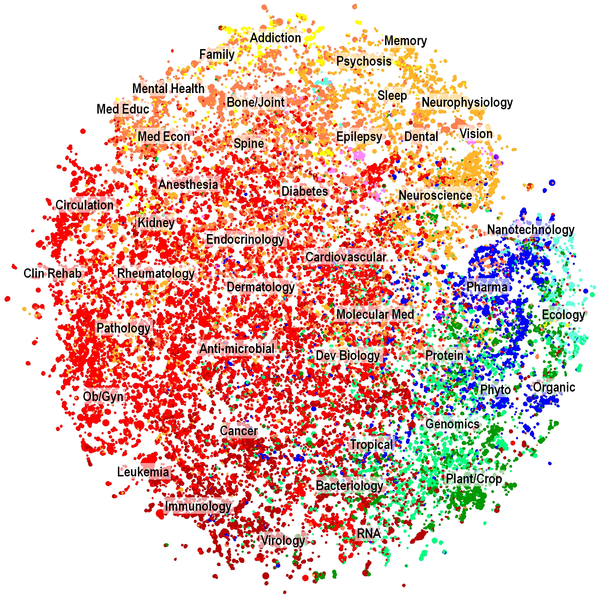
\includegraphics[width=\textwidth]{images/medical.png}
    \end{center}
    \end{column}
  \end{columns}

\end{frame}

% ============================================== %

\section{Multidimensional Scaling}

% ============================================== %

\begin{frame}

\begin{center}
{\Large Multidimensional Scaling}
\end{center}

\end{frame}

\begin{frame}{Идея метода}

Перейти в пространство меньшей размерности так, чтобы расстояния между объектами в новом пространстве были подобны расстояниям в исходном пространстве.

\end{frame}

\begin{frame}{Обозначения}

\begin{itemize}
\item $\mathbf{x}_i \in \mathcal{X} \subset R^D$ -- объекты в исходном многомерном пространстве
\item $\delta_{ij}$ -- расстояние между $\mathbf{x}_i$ и $\mathbf{x}_j$
\item $\mathbf{x}_i \in \mathcal{Y} \subset R^E$ -- объекты в целевом пространстве ($E=2$ или $E=3$)
\item $d_{ij}$ -- расстояние между $\mathbf{y}_i$ и $\mathbf{y}_j$
\end{itemize}

\begin{center}
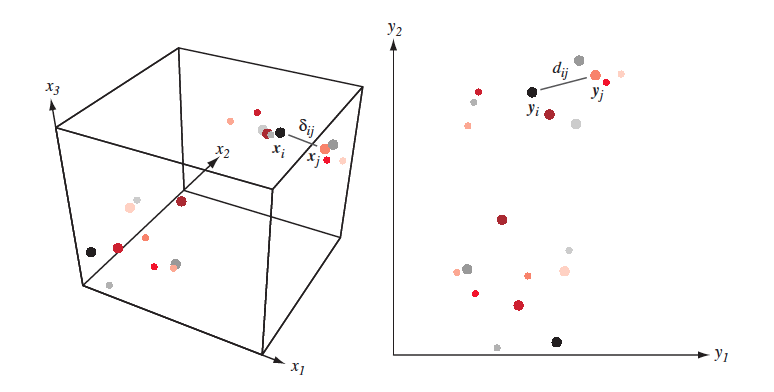
\includegraphics[scale=0.35]{images/mds.png}
\end{center}

\end{frame}

\begin{frame}{Критерии}

Выбираем кофигурацию $\mathbf{y}_i$, соответствующую минимуму критерия
\[
J_{ee} = \frac{\sum_{i < j} (d_{ij} - \delta_{ij})^2} {\sum_{i < j} \delta_{ij}^2}
\]
\[
J_{ff} = \sum_{i < j} \frac{(d_{ij} - \delta_{ij})^2}{\delta_{ij}^2}
\]
\[
J_{ef} = \frac{1} {\sum_{i < j} \delta_{ij}}\sum_{i < j} \frac{(d_{ij} - \delta_{ij})^2}{\delta_{ij}}
\]

\end{frame}

\defverbatim[colored]\gd{%
\begin{lstlisting}[tabsize=4,basicstyle=\ttfamily]
function gd(grad, a0, epsilon):
	initialise eta(k)
	k = 0
	a = a0	 
	do:
		k = k + 1
		a = a - eta(k) grad(a)
	until |eta(k) grad(a)| < epsilon
	return a
\end{lstlisting}
}

\begin{frame}{Градиентный спуск}

Требуется найти минимум функции $f(\mathbf{a})$, при этом
\begin{enumerate}
\item мы умеем вычислять градиент функции $\nabla f(\mathbf{a})$
\item задана начальная точка $\mathbf{a}_0$
\item выбрана функция learning rate $\eta(k)$
\end{enumerate}

\gd

(\href{http://vis.supstat.com/2013/03/gradient-descent-algorithm-with-r/}{демо})

\end{frame}

\begin{frame}{Градиенты критериев}

\[
\nabla_{\mathbf{y}_k}J_{ee} = \frac{2} {\sum_{i < j} \delta_{ij}^2} \sum_{j \neq k} (d_{kj} - \delta_{kj}) \frac{\mathbf{y}_k - \mathbf{y}_j}{d_{kj}}
\]
\[
\nabla_{\mathbf{y}_k} J_{ff} = 2 \sum_{j \neq k} \frac{d_{kj} - \delta_{kj}}{\delta_{kj}^2} \frac{\mathbf{y}_k - \mathbf{y}_j}{d_{kj}}
\]
\[
\nabla_{\mathbf{y}_k} J_{ef} = \frac{2} {\sum_{i < j} \delta_{ij}} \sum_{j \neq k} \frac{d_{kj} - \delta_{kj}}{\delta_{kj}} \frac{\mathbf{y}_k - \mathbf{y}_j}{d_{kj}}
\]

\end{frame}

\begin{frame}{Результаты применения}

\end{frame}

% ============================================== %

\section{T-SNE}

% ============================================== %

\begin{frame}

\begin{center}
{\Large T-SNE}
\end{center}

\end{frame}

\begin{frame}{Идея метода}

Та же, что в MDS, но определяется необычная (вероятностная) схожесть между объектами в исходном и целевом пространствах, а также критерий оптимизации.

\vspace{1em}
Схожесть между объектами $\mathbf{x}_i$ и $\mathbf{x}_j$ $\sim$ вероятность того, что $\mathbf{x}_i$ ``выберет'' $\mathbf{x}_j$ из остальных соседей, будучи центром некоторого нормального распределения.

\end{frame}

\begin{frame}{Схожесть между объектами}

В исходном пространстве
\[
p(j | i) = \frac{\exp(-\|\mathbf{x}_j-\mathbf{x}_i\|^2/{2 \sigma_i^2})}{\sum_{k \neq i}\exp(-\|\mathbf{x}_k-\mathbf{x}_i\|^2/{2 \sigma_i^2})}
\]

В целевом пространстве
\[
q(j | i) = \frac{\exp(-\|\mathbf{y}_j-\mathbf{y}_i\|^2)}{\sum_{k \neq i}\exp(-\|\mathbf{y}_k-\mathbf{y}_i\|^2)}
\]

\end{frame}

\begin{frame}{Критерий оптимизации}

\begin{block}{Дивергенция Кульбака-Лейблера}
Насколько распределение $P$ отличается от распределения $Q$?
\[
KL(P \| Q) = \sum_i P(z) \log \frac{P(z)}{Q(z)}
\]
\end{block}

Критерий
\[
J_{SNE} = \sum_i KL(P_i \| Q_i) = \sum_i \sum_j p(j | i) \log \frac{p(j | i)}{q(j | i)} \rightarrow \min_{\mathbf{y}_1, \ldots, \mathbf{y}_n}
\]
Градиент
\[
\nabla_{\mathbf{y}_i} J_{SNE} = 2 \sum_j \left(p(j | i) - q(j | i) + p(i | j) - q(i | j) \right) (\mathbf{y}_i-\mathbf{y}_j)
\]

\end{frame}

\begin{frame}{Параметры алгоритма}

\begin{exampleblock}{Идея}
В областях высокой плотности выбрать $\sigma_i$ маленьким, а в областях низкой плотности -- большим.
\end{exampleblock}
\[
Perp(P_i) = 2^{H(P_i)}, \quad H(P_i) = - \sum_j p(j | i) \log p(j | i)
\]
На практике выбираем фиксированное perplexity в интервале $(5, \; 50)$.


\end{frame}

\begin{frame}{T-SNE}

Недостатки SNE
\begin{itemize}
\item Трудно оптимизировать критерий
\item ``Crowding problem''
\end{itemize}

\vspace{1em}
Отличия T-SNE от SNE
\begin{itemize}
\item Использует симметризованный критерий с более простым градиентом
\item В целевом пространстве схожесть основана на t-распределении, а не на распределении Гаусса
\end{itemize}

\end{frame}

\begin{frame}[plain]
\begin{center}
{\Large Вопросы}
\end{center}
\end{frame}

\end{document}